%\documentclass[spanish,12pt,a4paper,titlepage,twoside,openright]{scrbook}
\documentclass[12pt,a4paper,titlepage]{report}
%\usepackage[latin1]{inputenc}
\usepackage[utf8]{inputenc}
\usepackage{graphicx}
\usepackage{subfig}
\usepackage{float}
\usepackage{wrapfig}
\usepackage{multirow}
\usepackage{caption}
\usepackage[spanish,es-nodecimaldot]{babel}
\usepackage[dvips]{hyperref}
\usepackage{amssymb}
\usepackage{listings}
\usepackage{epsfig}
\usepackage{amsmath}
\usepackage{array}
\usepackage[table]{xcolor}
\usepackage{multirow}
\usepackage{hhline}
\usepackage{cancel}
\usepackage{fancyvrb}

\usepackage[framed,numbered,autolinebreaks,useliterate]{mcode}

\usepackage[Sonny]{fncychap}
%\usepackage[Glenn]{fncychap}
%\usepackage[Conny]{fncychap}
%\usepackage[Rejne]{fncychap}
%\usepackage[Bjarne]{fncychap}

\usepackage{subfiles}
\usepackage{framed}
\usepackage{appendix}
\setlength{\topmargin}{-1.5cm}
\setlength{\textheight}{25cm}
\setlength{\oddsidemargin}{0.3cm} 
\setlength{\textwidth}{15cm}
\setlength{\columnsep}{0cm}
%\setkomafont{disposition}{\normalfont\bfseries}
\captionsetup{tablename=Tabla}

\ChNameVar{\bfseries\LARGE\sf}\ChNumVar{\fontsize{62}{65}\selectfont}
\ChTitleVar{\bfseries\LARGE\sf} \ChRuleWidth{2pt} \ChNameAsIs
\ChTitleAsIs
\renewcommand\FmN[4]{}
\newcommand{\HRule}{\rule{\linewidth}{0.5mm}}
\newcommand{\bs}{\boldsymbol}

\fvset{frame=single,framesep=1mm,fontfamily=courier,fontsize=\scriptsize,numbers=left,framerule=.3mm,numbersep=1mm,commandchars=\\\{\}}

\begin{document}

\begin{titlepage}
\begin{center}
\vspace{3cm}
\textsc{\LARGE Facultad de Ingenier\'ia de la Universidad de la Rep\'ublica}\\[1.5cm]
\vspace{2cm}
\textsc{\Large Introducción al Reconocimiento de Patrones  \\[1cm]  Curso 2013}\\[0.5cm]
\vspace{2cm}
% Title
\vspace{.7cm}
\HRule \\[1cm]
{ \huge \bfseries Proyecto final}\\[0.4cm]
\HRule \\[1cm]
\vspace{2cm}
% Author and supervisor

\begin{center}
\begin{tabular}{p{.5\textwidth}p{.5\textwidth}}
\emph{Autores:} & \hfill \emph{Tutores:}\\
Josué Luiz \textsc{Ñuñez} &  \hfill Federico \textsc{Lecumberry}\\
Mat\'ias \textsc{Tailani\'an} & \hfill Ignacio \textsc{Ramirez}
\end{tabular}
\end{center}

\vspace{1cm}

\vfill
\begin{figure} [h!]
\centering
\subfloat{
\includegraphics[width=0.25\textwidth]{./pics/logoIIE_transparente.png}}\hspace{1cm}
\subfloat{
\includegraphics[width=0.15\textwidth]{./pics/logo_fing_transparente.png}}\hspace{1cm}
\subfloat{
\includegraphics[width=0.15\textwidth]{./pics/logo_udelar.png}}
\end{figure}

% Bottom of the page
{\large \today}
\end{center}
\end{titlepage}

\tableofcontents

\chapter{Introducción}
El objetivo principal del proyecto es la investigación en técnicas que permitan contribuir con la predicción de fertilidad de rodeo lechero y la calidad de la carne integrando técnicas de reconocimiento de patrones sobre datos de alta dimensión.\\

A lo largo de los años se ha intentado relacionar ciertas características fenotípicas del ganado bovino con algunos indicadores genéticos. Es un problema actualmente abierto de gran interés mundial y Uruguay, siendo un país esencialmente ganadero, no puede estar ajeno. Desde hace varios años se viene desarrollando una línea de investigación relacionada con la genética molecular de la calidad de la carne bovina en el área de Genética de la Facultad de Veterinaria. Se ha realizado un abordaje desde diferentes puntos de vista, como la caracterización de genes conocidos en rodeos vacunos de nuestro país, o la búsqueda y análisis de nuevos genes asociados a la calidad de carne tanto bovina como ovina \cite{bib:eileen}.\\

Obtener una correlación entre la información genética y la capacidad reprodutiva de bovinos, el impacto en la calidad de la leche y de la carne de los animales de nuestros rodeos tendría un alto impacto en la producción. A lo largo de los últimos años en Facultad de Veterinaria se han creado bases de datos con información fenotípica y genotípica relacionada conla calidad cárnica y la fertilidad bovina aplicada a la producción lechera. En esta oportunidad se trabajará con una base de datos confeccionada en nuestro país durante el año 2009, provista por la veterinaria Dra. Ana Meikle.

\chapter{Base de datos}
Para lo que sigue de este trabajo es importante conocer la base de datos con la que se trabajará, y realizar una breve descripción de las características relevantes.\\

La base de datos consta de información de un seguimiento realizado durante 9 meses sobre 891 vacas de 7 tambos diferentes y consiste en las características detalladas a continuación.

\section{Características fenotípicas}
\begin{itemize}
	\item Edad.
	\item Condición corporal (BCS) desde 30 días previos al parto hasta 120 días pos-parto, con una frecuencia de al menos una vez cada 30 días. Se utilizó la escala de 5 puntos (1=flaca, 5= gorda).
	\item Cantidad de partos (Cantidad de lactancias). Es un indicador importante que tiene que ver con la historia y desgaste de la vaca.
	\item Anestro: es la cantidad de días que pasaron desde el parto hasta el reinicio. El reinicio se define como el día en que la progesterona aumenta a un nivel determinado, indicando que la vaca volvió a ciclar.
	\item Intervalo entre partos. Es la cantidad de días que pasan entre 2 partos consecutivos (válido solamente para vacas multíparas). Para maximizar la producción de leche lo que se busca es que la vaca quede peñada una vez al año, es decir un intervalo entre partos de 365 aproximadamente.
	\item Secado: la cantidad de días que pasan entre el último día que se le saca leche a la vaca y el parto. Es válido solo para vacas multíparas. Es un indicador de cuanto tiempo se dejó descansar a la vaca antes del parto. Cuanto más tiempo tiene, se prepara el cuerpo y llega en mejor forma.
	\item Servicios: Cantidad de inceminaciones realizadas para lograr la preñez.
	\item Concentración de progesterona hasta los 60 días posparto.
	\item Promedio de cantidad de grasa en la leche durante los primeros 100 días posparto.
	\item Promedio de cantidad de leche durante los primeros 100 días posparto.
\end{itemize}

\section{Características genotípicas - Determinación de polimorfismos (SNPs)}
Se extrajo ADN y se obtuvieron muestras de buena calidad. En la figura \ref{fig:genotipo} se muestra el procedimiento realizado para caracterizar el gen IGF-I bovino en 3 clases: ``AA'', ``AB'' y ``BB''. 

\begin{figure}[H]
	\centering 
	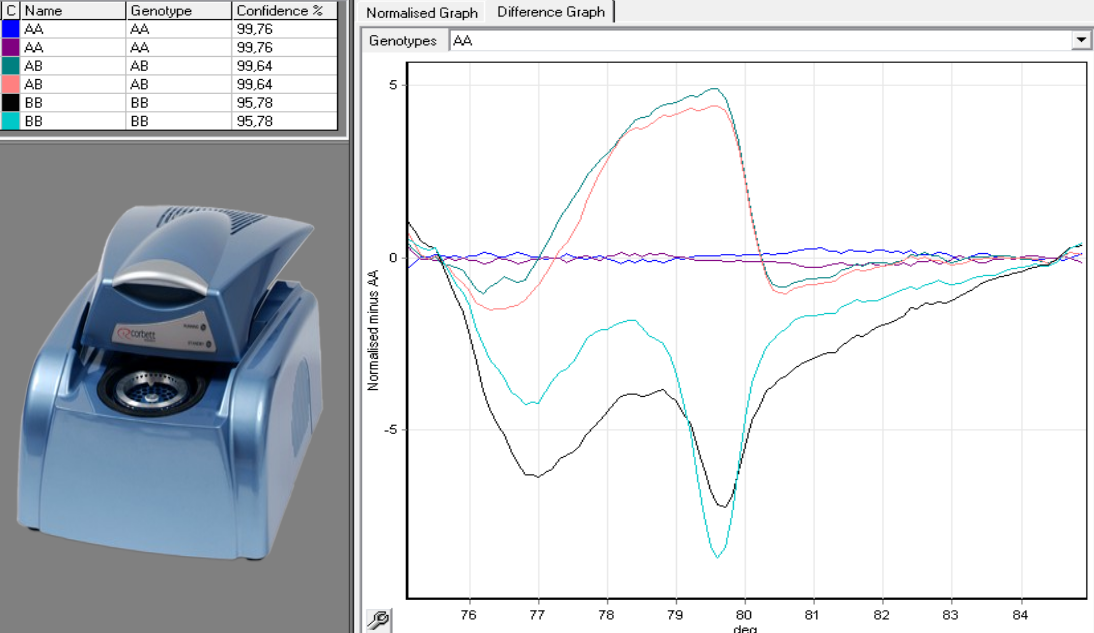
\includegraphics[width=.8\textwidth]{./pics/genotipos.png}
	\caption{Determinación del genotipo}
	\label{fig:genotipo}
\end{figure}

El eje de las ordenadas muestra la fluorescencia normalizada al genotipo ``AA''. Se puede observar que el genotipo ``AB'' se encuentra por encima del genotipo normalizado, mientras que el genotipo ``BB'' por debajo.

\section{Resumen}
En primer lugar fue necesario entender e interiorizarse con la base de datos, los conceptos y la terminología específica del problema. La lectura e interpretación de los datos no resulta para nada sencilla, por lo que se realizaron dos reuniones con la Dr. Ana Meikle, encargada de la investigación que llevó a cabo la confección de la base asociada a la producción de leche y fertilidad del ganado bovino. En ambas reuniones se buscó depurar la base con el fin de quitar información repetida y no relevante para el estudio. También se estableció un orden de relevancia en las características fenotípicas.\\

En resumen contamos con una base de datos acotada y ``limpia'' con varias características fenotípicas que se quieren correlacionar con los genotipos de cada individuo. En particular se abordará el problema como un trabajo de clasificación, tomando los genotipos como clases.

\chapter{Técnicas utilizadas}
La mayoría de los algoritmos de \emph{machine learning} seleccionan los atributos apropiados para realizar sus decisiones. Por ejemplo los métodos de árbol de desición eligen en cada paso la característica que mejor separa en clases. Cuantas más características tengamos, en teoría tendremos más poder de discriminación, pero en la práctica no ocurre así. Agregar información irrelevante o características distractivas, confunde a los algorimos de machine learning. Está probado que el número de instancias necesarias para entrenamiento para producir un cierto nivel de performance crece exponencialmente con la cantidad de atributos irrelevantes.\\

Dado el efecto negativo de las características irrelevantes es muy común en muchos algoritmos de \emph{machine learning} que se realice una etapa de selección de características donde se eliminen las irrelevantes. La mejor manera de realizar una selección de características es manual, adquiriendo un amplio conocimiento del problema en cuestión y logrando interpretar cada una de las características. Sin embargo es posible realizar una selección con algoritmos automáticos que resultan muy útiles. Reducir la dimensionalidad de los datos puede mejorar la performance de los algoritmos, además de reducir la complejidad del problema y bajar los requerimientos de capacidad de cómputo. Por esta razón se realizará una etapa de selección automática de características previa a la clasificación, como se explicará más adelante.\\ 

En una primera etapa de análisis sobre la base de datos se ataca el problema con los clasificadores \textbf{C4.5}, \textbf{Naive Bayes} y \textbf{K-NN}. \\

El algoritmo \textbf{C4.5} se utiliza para generar un árbol de desición que puede ser utilizado para clasificación. Por la naturaleza de los árboles, es un algoritmo no paramétrico, por lo que resulta robusto ante \emph{outliers}.\\

\textbf{Naive Bayes} es un clasificador basado en la aplicación del teorema de Bayes. No particiona el espacio de instancias e ignora de forma robusta a las características irrelevantes. Asume por diseño que todas las características son independientes entre si, y paga un precio muy alto cuando hay características redundantes.\\

El algoritmo \textbf{k-NN} (k-nearest neighbors) es un algoritmo de clasificación supervizado no paramétrico que pedice la clase de las instancias basado en los \emph{k} vecinos más cercanos. Es un algoritmo muy sensible a la propia estructura de los datos. Cuando $k\rightarrow \infty$, el algoritmo asegura una tasa de error no superior al doble de la tasa de error de Bayes (mínimo alcanzable dada la distribución de los datos).\\

Con esta batería de clasificadores se cubre un amplio espectro y se utilizan algunos de los algoritmos más utilizados para problemas de reconocimiento de patrones.\\

Para analizar los resultados se utilizan las implementaciones provistan en el software \textbf{Weka} \cite{bib:weka}.

\section{Primera etapa}
Se utiliza el clasificador compuesto \verb AttributeSelectedClassifier  que aplica una técnica de selección de características antes de entrenar al clasificador. Se logra entonces una reducción de la dimensionalidad. La estrategia elegida para la selección de características se realiza utilizando el enfoque \verb wrapper , que evalúa el set de atributos utilizando un esquema de aprendizaje y utiliza validación cruzada para estimar la precisión del esquema de aprendizaje. El clasificador utilizado para estimar esta precisión es un árbol de decisión \textbf{C 4.5}.\\

En todos los casos se utilizó validación cruzada con 10 subconjuntos.\\

Una vez hecha la extracción de características, y así la reducción de dimensionalidad, se estudia el desempeño de diferentes clasificadores.

\subsection{Naive Bayes}


\subsection{C 4.5}

\subsection{K-nn}



\section{Segunda etapa - masajeo de datos}

\subsection{Naive Bayes}

\subsection{C 4.5}

\subsection{K-nn}





	\section{PCA}
	
	\section{LDA?}
	
	\section{NN?}
	
	\section{SVM?}

\chapter{Conclusiones}






\begin{thebibliography}{99}
\begin{small}

\bibitem{bib:eileen}Eileen Armstrong Reborati, \emph{Detección y análisis de genes asociados a la calidad de la carne en bovinos}, Tesis de doctorado, Madrid, 2011.
\bibitem{bib:weka}Mark Hall, Eibe Frank, Geoffrey Holmes, Bernhard Pfahringer, Peter Reutemann, Ian H. Witten (2009); The WEKA Data Mining Software: An Update; SIGKDD Explorations, Volume 11.
\bibitem{bib:REML}Meyer, K. (2007). WOMBAT – A tool for mixed model analyses in quantitative genetics by REML, J. Zhejiang Uni.

\end{small}
\end{thebibliography}





\end{document}

\begin{wrapfigure}{l}{0.6\textwidth}
	\vspace{-20pt}
	\begin{center}
		\includegraphics[width=0.45\textwidth]{./pics/.pdf}
	\end{center}
	\vspace{-20pt}
	\caption{}
	\label{}
	\vspace{-10pt}
\end{wrapfigure}


\begin{figure} [H]
\centering
  \subfloat[Características 1]{\label{fig:c1} 
  		\includegraphics[width=.5\textwidth]{./pics/carac1.pdf}} 
  \subfloat[Características 2]{\label{fig:c2} 
  		\includegraphics[width=.5\textwidth]{./pics/carac2.pdf}} \\
  \caption{Histogramas de las características} 
  \label{fig:c1yc2}
\end{figure}


\begin{figure}[H]
	\centering 
	\includegraphics[width=.8\textwidth]{./pics/ej2_voronoi_12_coloreada.pdf}
	\caption{Voronoi - Características 1 y 2}
	\label{fig:voronoi12}
\end{figure}